\documentclass[xcolor=dvipsnames,aspectratio=169]{beamer} % if you use \onslide or overprints
%\documentclass[xcolor=dvipsnames,aspectratio=169,handout]{beamer} % if you don't use \onslide and overprints

% CREATED BY: Mattia Secchi

%\documentclass[handout]{beamer}
% Use this mode to create an handout version of the presentation to distribute to the audience:
% every "frame" will be 1 slide only, so the <onslide> commands will not influence the number of
% pages printed

%% --Packages--

\usepackage{graphicx}
%\usepackage{amsmath}
\usepackage{hyperref}
\usepackage{float}
\usepackage{geometry}
\usepackage{tikz}
\usepackage{xcolor}
%\usepackage[italian]{babel}
\usepackage{fancyhdr}

%\deftranslation[to=italian]{Example}{Esempio} %for example translation to "esempio" if needed

\mode<presentation>

%%%%%%%%%%%%%%%%%%%%%%%%%%%%%%%%%%%%%%%%%%%%%%%%%%%%%%%%%%%%%%%%%%%%%%%%%%%%%%%%%%%%%%%%%%%%%
%% Some settings...

%gets rid of bottom navigation bars and page numbers
%\setbeamertemplate{footline}{}

%gets rid of navigation symbols
\setbeamertemplate{navigation symbols}{}

%setting arev font
\usepackage{arev}

%setting geometry of blocks and shadow
\setbeamertemplate{blocks}[rounded][shadow=true]

%RGB defining color if you want manual control of color, just like RedEurac ;)
\definecolor{RedEurac}{RGB}{208,77,42} 

%general colors and scheme, fg=font color and bg=background color
%just don´t put bg={} if you don´t want a background

\setbeamercolor{structure}{fg=RedEurac,bg=White} % color of structure (itemize, enumerate...)
\setbeamercolor{section in toc}{fg=RedEurac,bg=White} % table of contents color 
\setbeamercolor{block title example}{fg=RedEurac,bg=RedEurac} %title example color
\setbeamercolor{block body example}{fg=RedEurac,bg=White} %body example color
\setbeamercolor{block title itemize}{fg=RedEurac,bg=White} %title itemize color
\setbeamercolor{block body itemize}{fg=RedEurac,bg=White} %body itemize color 
\setbeamercolor{itemize item}{fg=RedEurac,bg=white} %item colour and enumerate color
\setbeamercolor{page number in head/foot}{fg=RedEurac} %page number color
\setbeamercolor{caption name}{fg=RedEurac} %caption name color

%override color of some specific element
\setbeamercolor{frametitle}{fg=RedEurac,bg=White!20,} %frametitle color and background color
\setbeamerfont{frametitle}{series=\bfseries}
\setbeamercolor{author}{fg=RedEurac,bg={}} %author color and background color
\setbeamercolor{date}{fg=White,bg={}} %date color and background color
\setbeamercolor{title}{fg=RedEurac,bg={}} %title color and background color
\setbeamercolor{subtitle}{fg=RedEurac,bg={}} %subtitle color and background color
\setbeamercolor{footline}{fg=RedEurac,bg={}}
\setbeamerfont{footline}{series=\small}
\setbeamercolor{footnote}{fg=RedEurac}

%gets rid of the rule in the footnotes
\renewcommand*\footnoterule{}

%positions the footnote for references inside the grey box at the bottom of the page
\setbeamertemplate{footnote}{
        \hspace*{3cm}%
        \insertfootnotemark
        \parbox[b][0.5cm]{7.5cm}{
            \insertfootnotetext%
        }%
}

%\pgfpagesuselayout{4 on 1}[a4paper,border shrink=5mm,landscape]
% Activate this option if you want to insert more than one slide in each page. Landscape
% is required only for 4 and 16 slides per page

\date{\today} %no date, just put one yourself if you want

% Author info
\newcommand{\authorsname}[1]{\textcolor{RedEurac}{
\underline{Mattia Secchi} \textsuperscript{1,2},
Grazia Barchi \textsuperscript{2}}}

\newcommand{\affiliationsname}[1]{\textcolor{RedEurac}{
\textsuperscript{1} University of Trento, Department of Industrial Engineering \\
\textsuperscript{2} Eurac Research, Institute for Renewable Energies}
}

\newcommand{\email}[1]{\textcolor{RedEurac}{\href{mailto:msecchi@eurac.edu}{\emph{msecchi@eurac.edu}}}}
\newcommand{\titledoc}[1]{\textcolor{RedEurac}{Peer-to-peer electricity sharing:}}
\newcommand{\subtitledoc}[1]{\textcolor{RedEurac}{\emph{maximising PV self-consumption through BESS \\ control strategies}}}

% Global background
\usebackgroundtemplate%
{%
    
\includegraphics[width=\paperwidth,height=\paperheight]{Background/middle.pdf}%
}

% Inserting logos in every page after title
\addtobeamertemplate{frametitle}{}{%
\begin{tikzpicture}[remember picture,overlay]
\node[anchor=south west] at (current page.south west) {
\includegraphics[height=0.4cm]{Logo/logo.png}};
\end{tikzpicture}}

% Note: to add an entry to summary you have to define sections with \section{•}

%____________________________________________________________________________________________%

\begin{document}

\color{Black} %setting global color of main text, you can set in here also a personalized color, like RedEurac

%%%%%%%%%%%%%%%%%%%%%%%%%%%%%%%%%%%%%%%%%%%%%%%%%%%%%%%%%%%%%%%%%%%%%%%%%%%%%%%%%%%%%%%%%%%%%
% TITLE SLIDE

{
\usebackgroundtemplate{
\includegraphics[width=\paperwidth]{Background/front.pdf}}

\begin{frame}[noframenumbering]

\vspace{130pt}

\Large \textbf{\titledoc} \\
\normalsize \subtitledoc \\ \\
\vspace{14pt}
\small \authorsname \\ \\
\small \affiliationsname

\end{frame}
}

{
\setbeamercovered{transparent} % to have the text on the sequential slides transparent

%%%%%%%%%%%%%%%%%%%%%%%%%%%%%%%%%%%%%%%%%%%%%%%%%%%%%%%%%%%%%%%%%%%%%%%%%%%%%%%%%%%%%%%%%%%%%
% SUMMARY SLIDE

% \begin{frame}[noframenumbering]{Summary}

% \begin{minipage}{0.5\paperwidth}
% \vspace{-24pt}
% \tableofcontents
% \end{minipage}
% \begin{minipage}{0.4\paperwidth}
% \vspace{-12pt}
% \centerline{
\includegraphics[height=5.5cm]{Logo/EEEIC_logo.jpg}}
% \end{minipage}
    
% \end{frame}

%inserting logos in every page after SUMMARY
\addtobeamertemplate{frametitle}{}{%
\begin{tikzpicture}[remember picture,overlay]
\node[anchor=north east] at (current page.north east) {
\includegraphics[height=1.5cm]{Logo/unitn.png}};
\end{tikzpicture}
}

% inserting page number with a specified format in the lower right corner
\addtobeamertemplate{navigation symbols}{}{%
    \usebeamerfont{footline}%
    \usebeamercolor[fg]{footline}%
    \hspace{1em}%
    \textcolor{RedEurac}{\insertframenumber/\inserttotalframenumber}
    \vspace{2pt}
}

%%%%%%%%%%%%%%%%%%%%%%%%%%%%%%%%%%%%%%%%%%%%%%%%%%%%%%%%%%%%%%%%%%%%%%%%%%%%%%%%%%%%%%%%%%%%%
% INTRODUCTION

\begin{frame}

\frametitle{Block+Vertical Minipages}

\vspace{-40pt}
    
    \begin{minipage}[t]{0.9\paperwidth}
    
    \onslide<1-3>{
    \begin{block}{Local Energy Community}
    "A cluster of houses performing some of the distribution system operator tasks, such as regulating power flows and participating in the electricity market. The main aim should not be generating profits but rather reducing the interaction with the grid.\footnote[frame]{EU Regulation: https://tinyurl.com/yd9dm6bd}"
    \end{block}
    }
    
    \end{minipage}
    \begin{minipage}[b]{0.9\paperwidth}
    
    \vspace{12pt}
    \onslide<2-3>{
    The EU wants:
    
    \begin{itemize}
        \item the customer to be fully involved in the energy system of the city
        \item electricity to be clean, affordable and available for everyone
    \end{itemize}
    }
    
    \onslide<3-3>{
    
    \begin{itemize}
        \item EU countries $\longrightarrow$ need to transpose the directive by June 2020
        \item Italy $\longrightarrow$ senate consultations on 26th March 2019
    \end{itemize}
    }
    
    \end{minipage}
    
\end{frame}

\begin{frame}[t]

\frametitle{Itemize+Minipage Horizontal}

\begin{minipage}{0.45\textwidth}

Peer-to-peer is a new concept allowing each user to:

\begin{overprint}
\begin{itemize}
    \onslide<1-1>{\item consume the extra production of the neighbours}
    \onslide<1-1>{\item sell its own extra production to the neighbour}
    \onslide<2-2>{\item store it own overproduction without selling to the grid}
    \onslide<3-3>{\item discharge the neighbours' battery to avoid buying from the grid}
\end{itemize}
\end{overprint}

\end{minipage}
\begin{minipage}{0.45\textwidth}

\begin{overprint}
    \onslide<1>{\includegraphics<1>[width=\textwidth]{Immagini/P2P1.png}}
    \onslide<2>{\includegraphics<2>[width=\textwidth]{Immagini/P2P3.png}}
    \onslide<3>{\includegraphics<3>[width=\textwidth]{Immagini/P2P2.png}}
\end{overprint}

\end{minipage}

\end{frame}

\begin{frame}[t]

\vspace{-20pt}

\frametitle{Full page picture}

\includegraphics[width=0.85\paperwidth]{Immagini/Grid2mod.png}

\end{frame}

\begin{frame}[t]

\frametitle{Vertical Pic+Itemize}

\begin{minipage}{0.35\textwidth}

\vspace{-24pt}

\begin{overprint}
  \onslide<1>\centerline{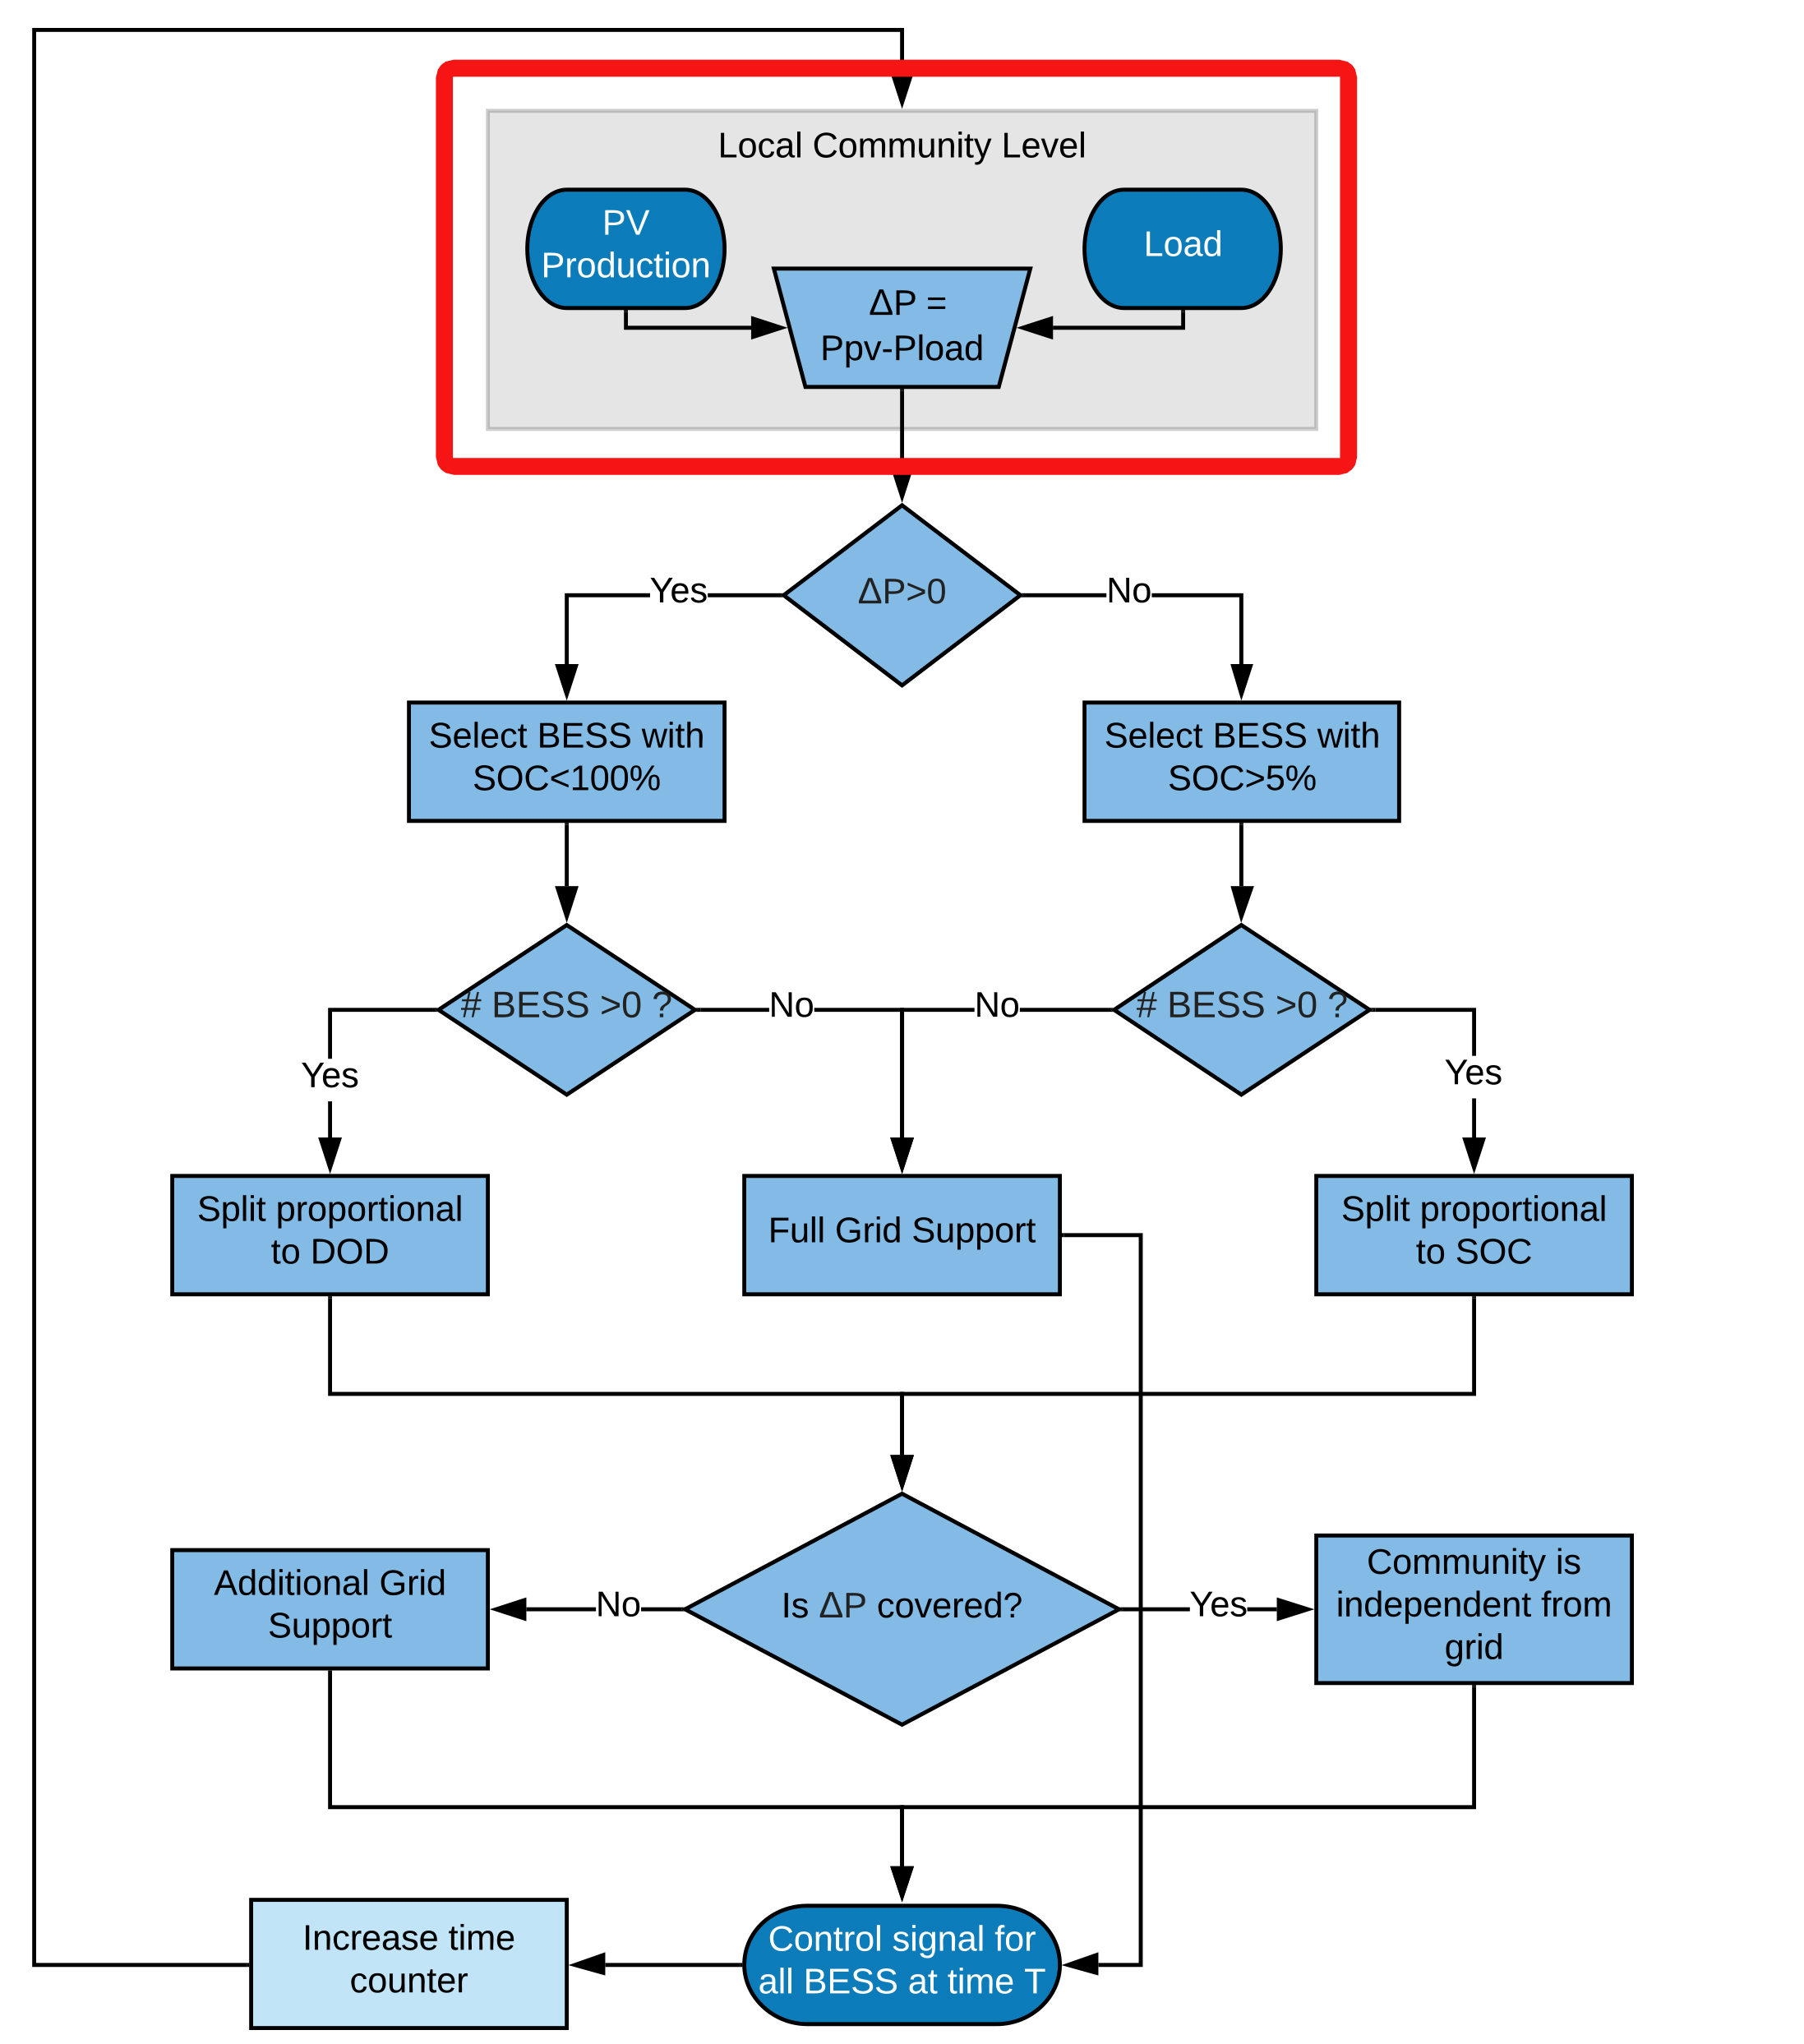
\includegraphics[width=\textwidth]{Immagini/SplitGeneral.jpg}}%
  \onslide<2>\centerline{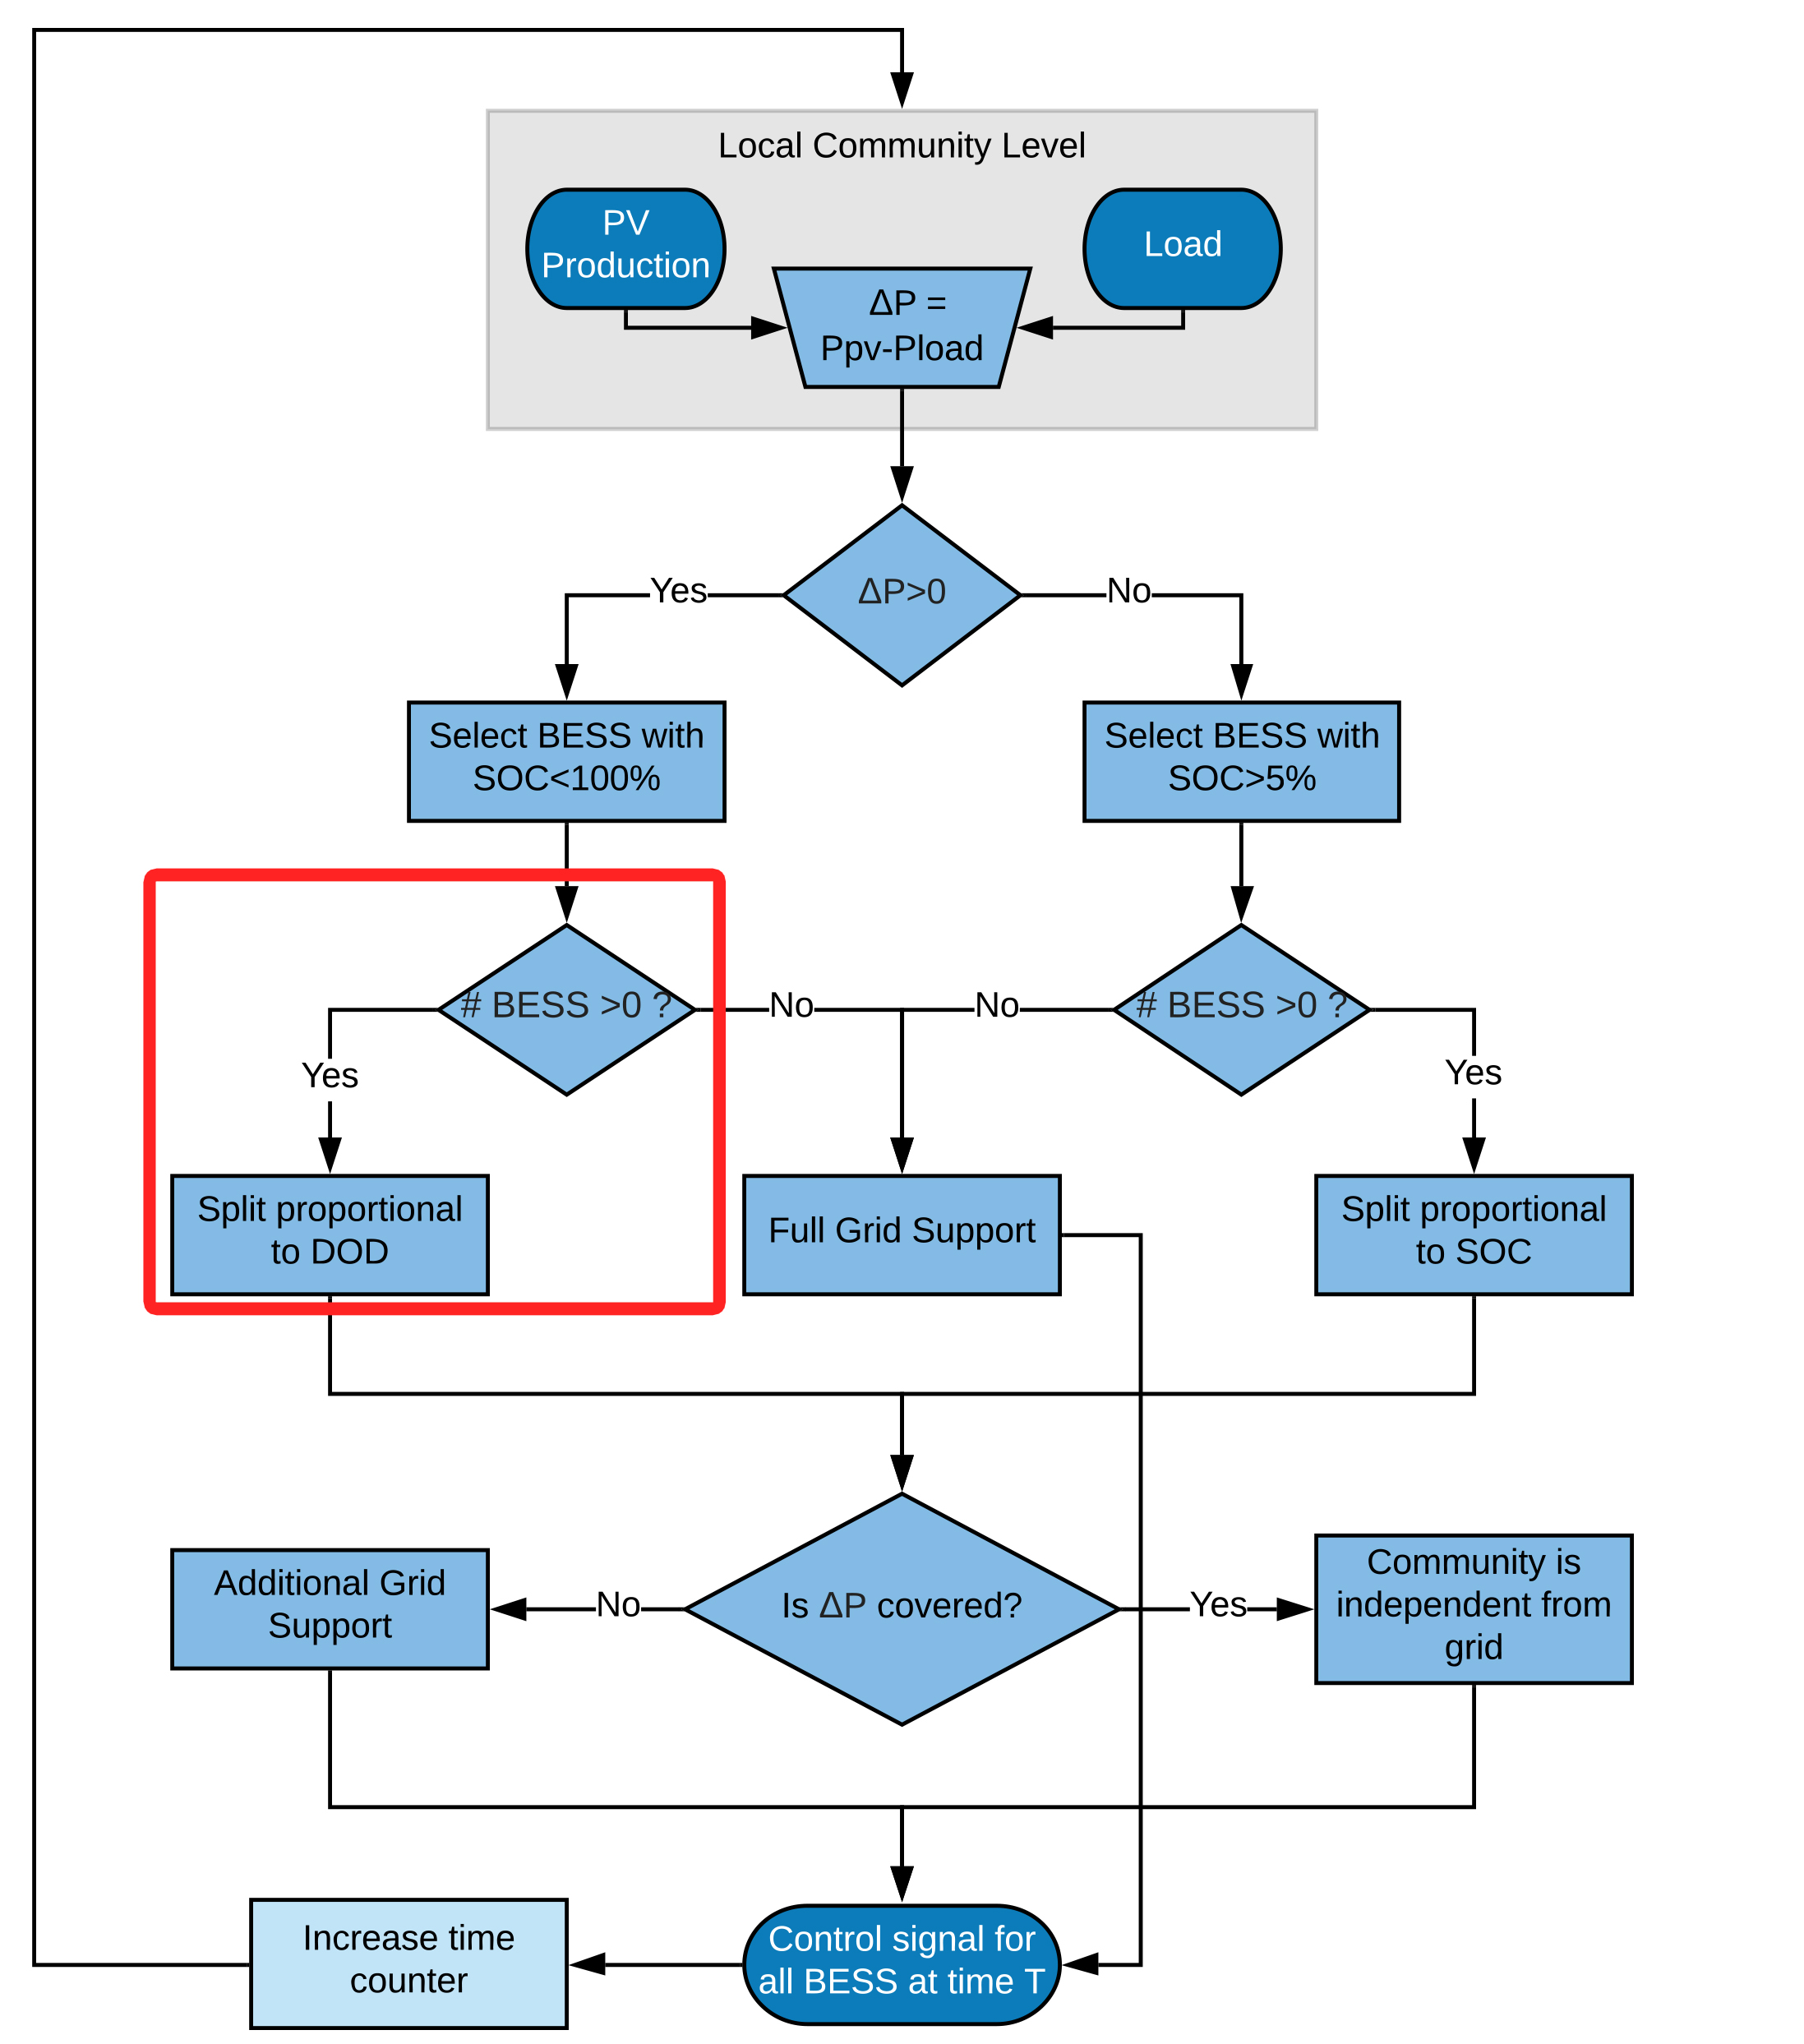
\includegraphics[width=\textwidth]{Immagini/SplitDOD.jpg}}%
  \onslide<3>\centerline{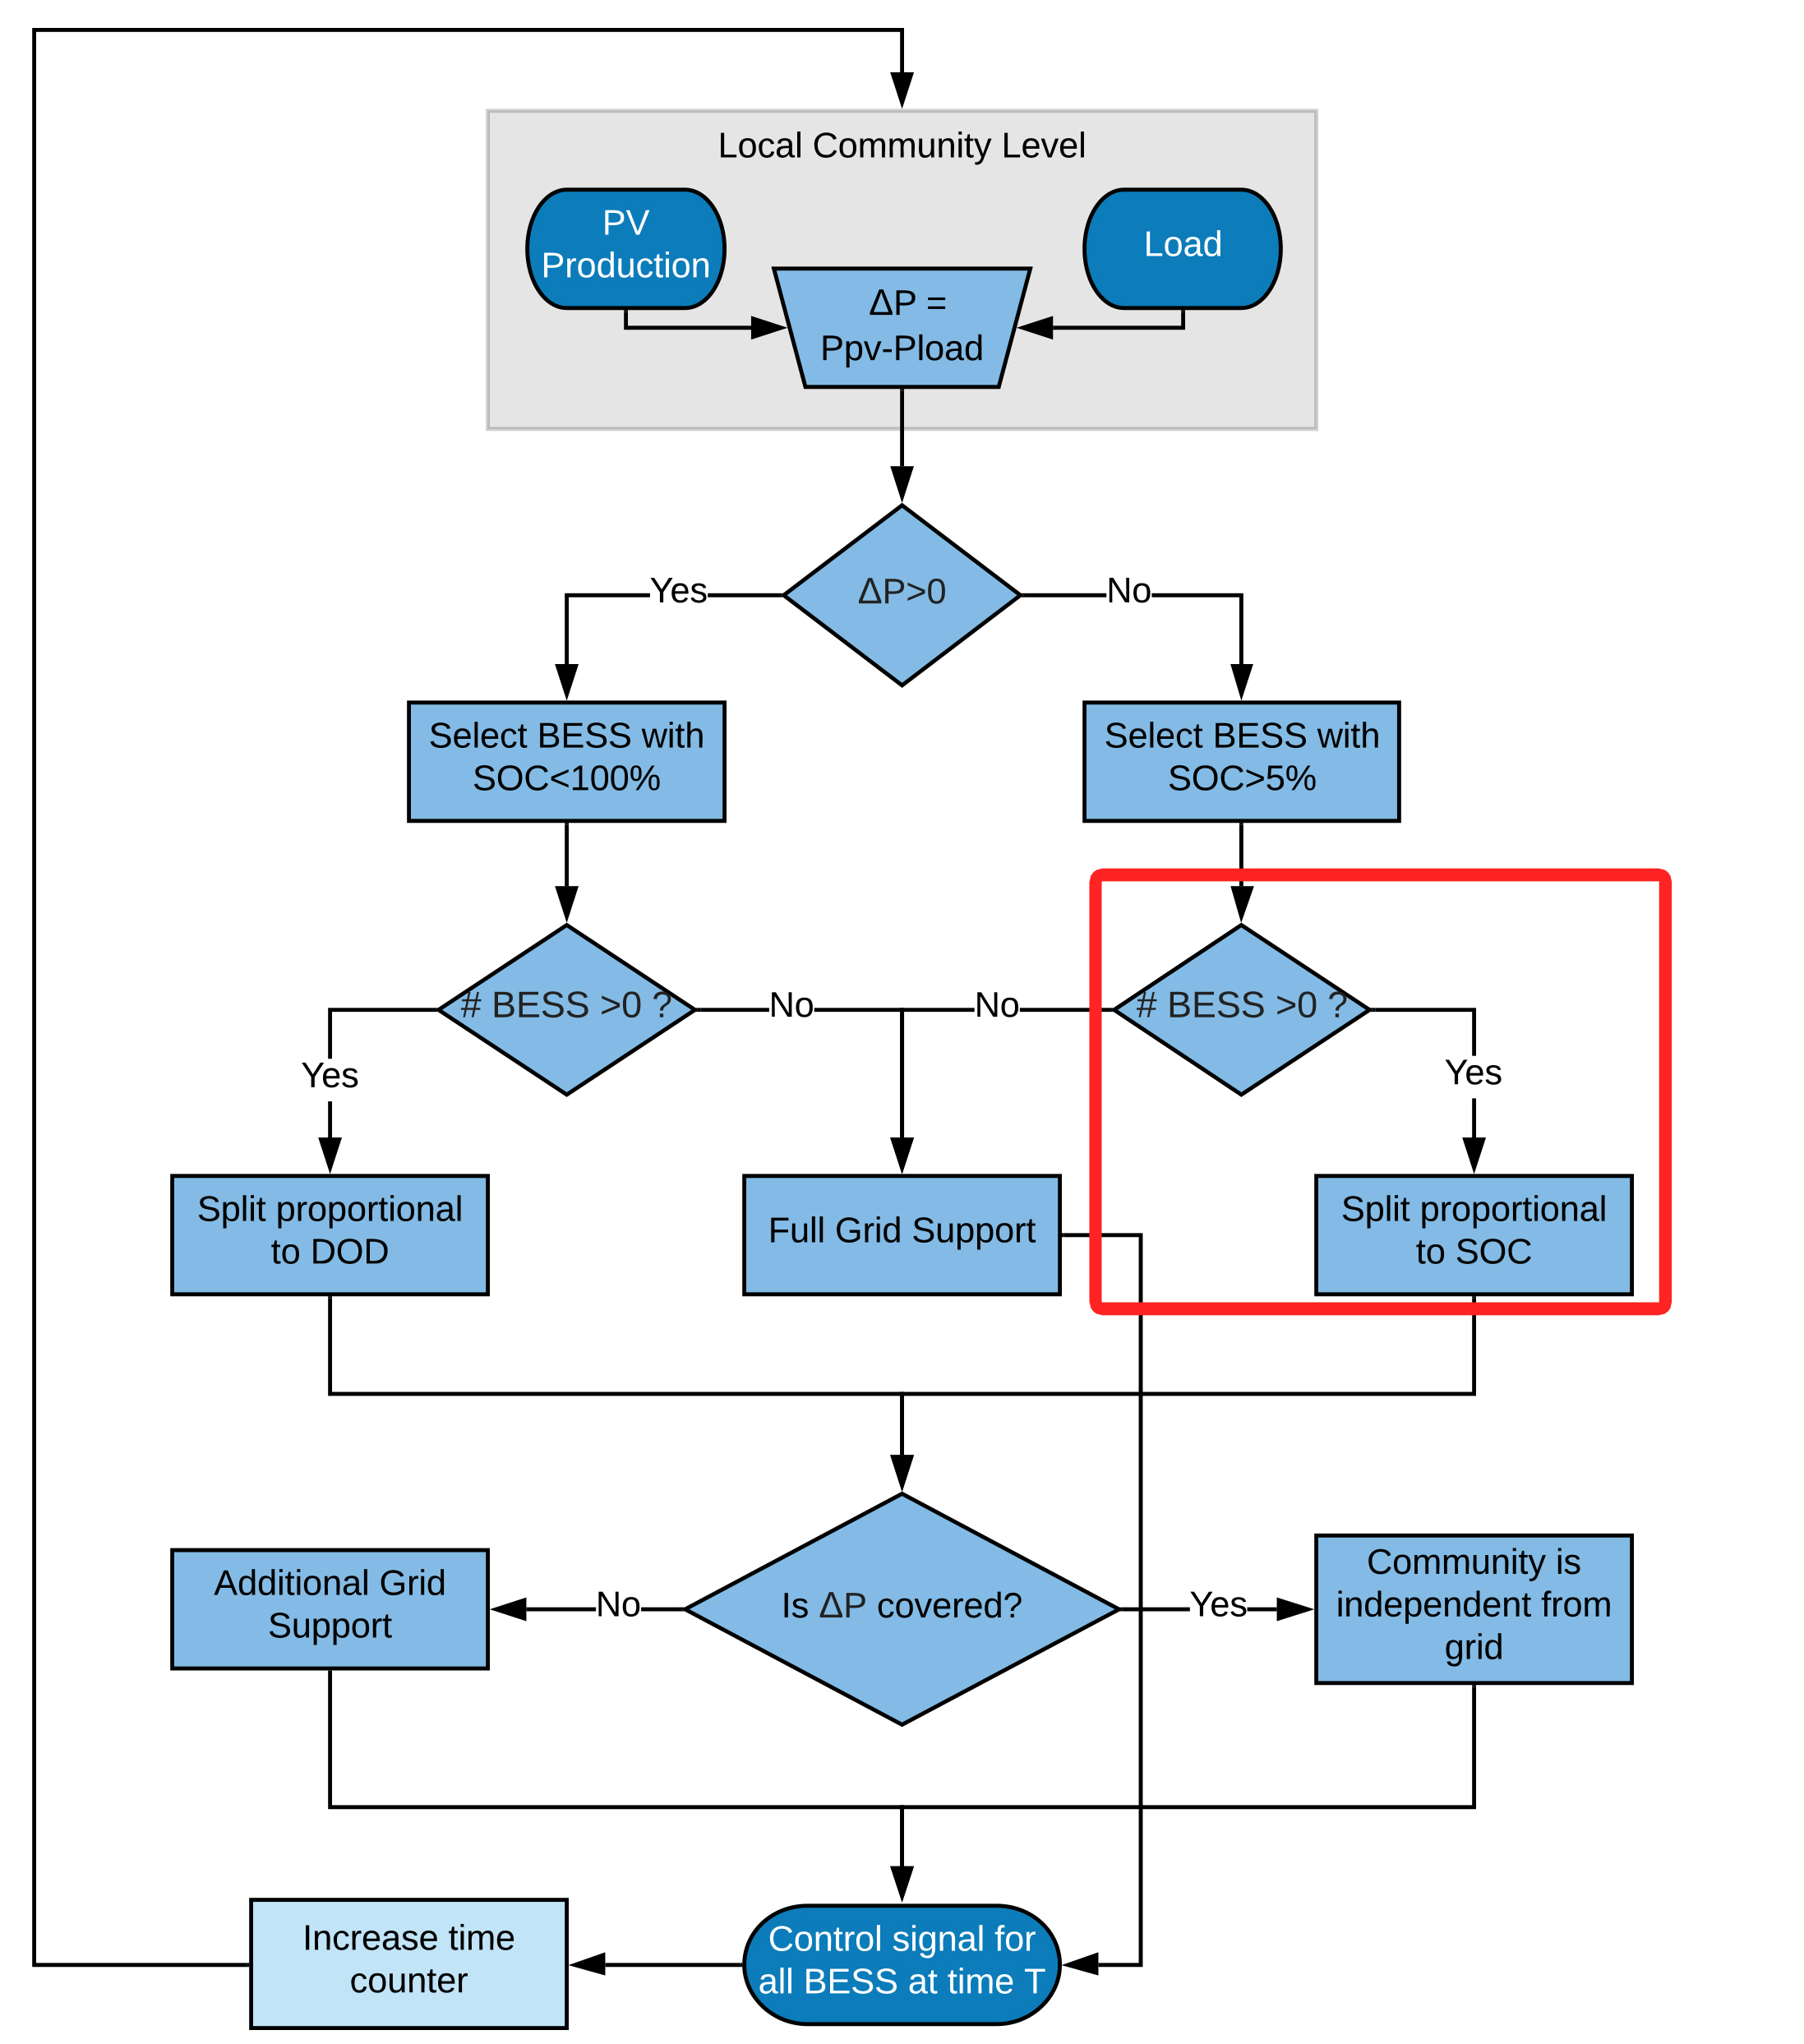
\includegraphics[width=\textwidth]{Immagini/SplitSOC.jpg}}%
\end{overprint}

\end{minipage}
\begin{minipage}{0.6\textwidth}

\begin{overprint}
\begin{itemize}

\onslide<1-1>{
\item Load to match/extra to sell for the whole community: \\ \vspace{12pt}
$P_{\Delta}(t) = \sum_{j=1}^N \left[P_{load,j}(t)-P_{PV,j}(t) \right]$ \vspace{12pt}
}

\onslide<2-2>{
\item Local community in overproduction: \\ \vspace{12pt}
$P_{toBESS,j}(t) = P_{\Delta}(t) \cdot \frac{DOD_j(t-\Delta t)}{\sum_{j=1}^N DOD_j(t-\Delta t)}$ \vspace{12pt}
}

\onslide<3-3>{
\item Local community in underproduction: \\ \vspace{12pt}
$P_{fromBESS,j}(t) = P_{\Delta}(t) \cdot \frac{SOC_j(t-\Delta t)}{\sum_{j=1}^N SOC_j(t-\Delta t)}$ \vspace{12pt}
}

\end{itemize}
\end{overprint}

\end{minipage}

\end{frame}

\begin{frame}[t]

\frametitle{Itemize+Pic or Table Hor.}

\begin{minipage}{0.5\textwidth}

\begin{overlayarea}{0.45\paperwidth}{\paperheight}
\begin{itemize}
    \onslide<1>{\item Tariffs based on time of the day and yearly consumption}
    \onslide<1>{\item Selling price is taken as the Italian SSP ("scambio sul posto").}
    \onslide<2>{\item PV cost: 1680 \euro \si{\per{\kilo\watt p}}}
    \onslide<2>{\item BESS cost: 715-1640 \euro \si{\per{\kilo\watt\hour}}}
    \onslide<3>{\item Irradiance and temperature profiles from Bozen (Italy).}
    \onslide<4>{\item Four houses, different synthetic consumption patterns.}
\end{itemize}
\end{overlayarea}

\end{minipage}
\begin{minipage}{0.5\textwidth}

\begin{overlayarea}{0.5\paperwidth}{\paperheight}

    \vspace{-12pt}
    \setbeamercovered{}
    \onslide<1-2>{\includegraphics<1-2>[width=0.8\textwidth]{Immagini/tariffs.pdf}
        \footnotesize{\textcolor{white}{Eurostat:} \\
        Eurostat:
        \url{https://ec.europa.eu/eurostat/cache/energy/prices/enprices.html?}
        }
    }
    \vspace{-40pt}
    \setbeamercovered{transparent}
    \onslide<3>{\vfill \vspace{-24pt} \includegraphics<3>[height=0.85\paperheight]{Immagini/irrtemp.png} \vfill}
    \vspace{40pt}
    \setbeamercovered{}
    \onslide<4>{\vfill \vspace{10pt} \footnotesize{
        \begin{tabular}{|c|c|} \hline
             \textbf{House 1} & \textbf{House 2} \\ \hline
             \SI{1.56}{\mega\watt\hour} & \SI{8.38}{\mega\watt\hour} \\ \hline
             Family, no children, & 2 Families, 3 children \\
             parents work. & each, parents work.\\ \hline
             \textbf{House 3} & \textbf{House 4}\\ \hline
             \SI{1.48}{\mega\watt\hour} & \SI{5.44}{\mega\watt\hour}\\ \hline
             Single woman, aged & 2 Single men, \\
             30-64, shift worker. &  over 65. \\ \hline
        \end{tabular}
        }
        \textcolor{white}{Load Profile Generator:} \\
        Load Profile Generator:
        \url{https://www.loadprofilegenerator.de/}
        \vfill
        }
\end{overlayarea}

\end{minipage}

\end{frame}

\begin{frame}[t]

\frametitle{Itemize+Raggedright Text}

\begin{minipage}{0.9\paperwidth}

\begin{itemize}
    \onslide<1-1>{\item $ SC= \frac{\sum_{j=1}^N \sum_{i=1}^{T} (E_{inst,i,j}+E_{toBESS,i,j})}{\sum_{j=1}^N \sum_{i=1}^{T} E_{PV,i,j}}$ \hfill Self Consumption \vspace{12pt}}
    \onslide<2-2>{\item $ SP= \frac{\sum_{j=1}^N \sum_{i=1}^{T} (E_{inst,i,j}+E_{fromBESS,i,j})}{\sum_{j=1}^N \sum_{i=1}^{T} E_{load,i,j}}$ \hfill Self Production \vspace{12pt}}
    \onslide<3-3>{\item $ GI_{togrid}=GI_{std}+GI_{max}+GI_{RR}$ \hfill Grid Indicator \vspace{12pt}}
    \onslide<4-4>{\item $SE_{CO2}=M_{CO_2,NOBESS}-M_{CO_2,BESS}$ \hfill Saved CO2 Emissions \vspace{12pt}}
    \onslide<5->{\item $PT = y|_{NPV(y)=0}$ \hfill Payback Time}
\end{itemize}

\end{minipage}

\end{frame}

\begin{frame}[t]

\frametitle{Pic+Bottom Minipage}

\vspace{-20pt}
\begin{minipage}[t]{0.8\paperwidth}
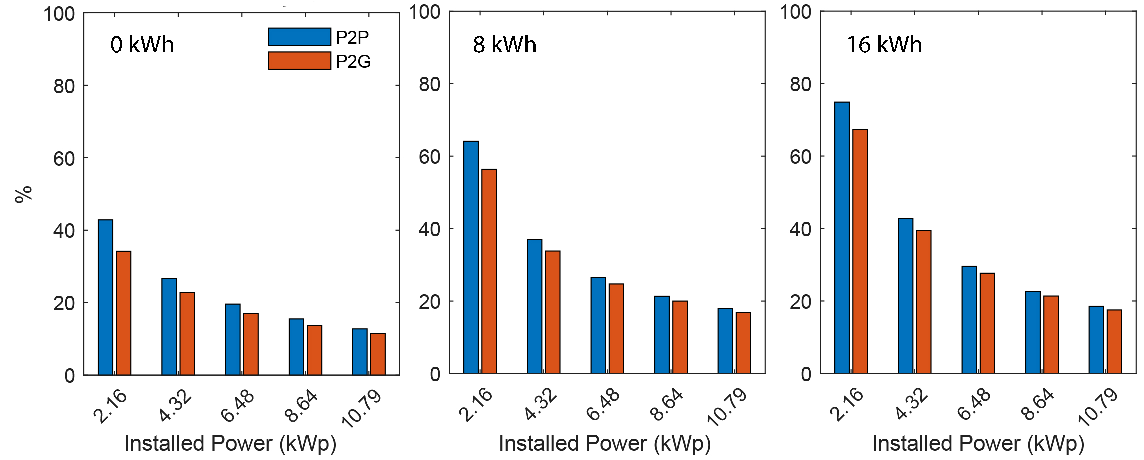
\includegraphics[height=0.55\paperheight]{Immagini/SCchoice1111.pdf}
\end{minipage}
\begin{minipage}[b]{0.8\paperwidth}
\vspace{8pt}
\begin{itemize}
    \onslide<1-2> \item The difference between P2G and P2P is more noticeable for undersized PV systems
    %\item the difference between P2G and P2P becomes less noticeable if the battery size increases
    \onslide<2-2> \item P2P prioritizes instantaneous SC rather than storage use, the battery size does not affect SC too much
    %\item SC decreases as installed power increases and increases as the battery size does
\end{itemize}

\end{minipage}

\end{frame}

} % this ends \setbeamercovered{transparent}

%%%%%%%%%%%%%%%%%%%%%%%%%%%%%%%%%%%%%%%%%%%%%%%%%%%%%%%%%%%%%%%%%%%%%%%%%%%%%%%%%%%%%%%%%%%%%
% CLOSURE SLIDE

{ % select a background for the closure slide
\usebackgroundtemplate{
\includegraphics[width=\paperwidth]{Background/end.pdf}}

\begin{frame}[noframenumbering]

\vspace{72pt}
\huge
\textbf{\textcolor{RedEurac}{Thank you \\
for your attention!}} \\
\vspace{24pt}
\Large \textbf{\textcolor{RedEurac}{Mattia Secchi}} \\
\textcolor{RedEurac}{University of Trento - Eurac Research} \\
\vspace{12pt}
\normalsize \email

\end{frame}
}

%%%%%%%%%%%%%%%%%%%%%%%%%%%%%%%%%%%%%%%%%%%%%%%%%%%%%%%%%%%%%%%%%%%%%%%%%%%%%%%%%%%%%%%%%%%%%
% BACKUP SLIDES

\begin{frame}[noframenumbering]{Box+Vertical Minipage}

\begin{minipage}[t]{0.9\paperwidth}

\vspace{-60pt}
\begin{block}{}
"Percentage of the PV production either stored in the batteries or instantaneously consumed by the houses."
\end{block}

\end{minipage}
\begin{minipage}[b]{0.9\paperwidth}

    \begin{equation*}
    SC= \frac{\sum_{j=1}^N \sum_{i=1}^{T} (E_{inst,i,j}+E_{toBESS,i,j})}{\sum_{j=1}^N \sum_{i=1}^{T} E_{PV,i,j}}
    \end{equation*}
    \begin{itemize}
    \item $E_{inst,i,j}$ = PV energy produced in house $j$ and instantaneously consumed at instant $i$
    \item $E_{toBESS,i,j}$ = PV energy stored in house $j$ battery at instant $i$
    \item $E_{PV,i,j}$ = instantaneous production at time $i$ and house $j$
    \end{itemize}

\end{minipage}

\end{frame}

\begin{frame}[noframenumbering]{Box+Left Empheq}

\begin{minipage}[t]{0.9\paperwidth}

\vspace{-45pt}
\begin{block}{}
"Impact of the storage capacity and P2P control on power flows from the community to the grid. \footnote[frame]{www.sciencedirect.com/science/article/pii/S0306261917303690}"
\end{block}

\end{minipage}
\begin{minipage}[t]{0.5\paperwidth}

\vspace{20pt}
    \begin{empheq}[right = \empheqrbrace]{align*}
    GI_{std} &= \frac{\sigma_{P_{togrid,BESS,0 \rightarrow T}}}{\sigma_{P_{togrid,noBESS,0 \rightarrow T}}} \\
    GI_{max} &= \frac{max(P_{togrid,BESS,0 \rightarrow T})}{max(P_{togrid,noBESS,0 \rightarrow T})} \\
    GI_{RR} &= \frac{\overline{RR}_{togrid,BESS,0 \rightarrow T}}{\overline{RR}_{togrid,noBESS,0 \rightarrow T}}
    \end{empheq}

\end{minipage} \hspace{-32pt}
\begin{minipage}[t]{0.3\paperwidth}

    \vspace{51pt}
    \begin{equation*}
    \longrightarrow GI_{inj}=GI_{std}+GI_{max}+GI_{RR} 
    \end{equation*}

\end{minipage}

\end{frame}

\begin{frame}[noframenumbering]{Equation+Itemize+Block}

\begin{minipage}{0.9\paperwidth}

    \vspace{-32pt}
    \begin{equation*}
    NPV_y = \sum_{i=1}^{y} \left[ CF_i \cdot \frac{1}{\left(1+\frac{i}{100} \right)^{DR_i}} \right]
    \end{equation*}
    \begin{itemize}
        \item $NPV_y$ = Net Present Value after "y" years from the installation of PV and BESS
        \item $DR_i$ = discount rate at year "i" after the investment
        \item $CF_y$ = cash flow at year "i" after the investment
    \end{itemize}
    \begin{block}{Payback Time (PT)}
    The year which nullifies the NPV, representing the "return time" for the investment.
    \end{block}
    
\end{minipage}

\end{frame}

\begin{frame}[noframenumbering]{Aligned equations+Picture Hor.}

\vspace{-12pt}

\begin{minipage}{0.4\paperwidth}

\begin{align*}
    I_{L,T} &= \cdot (I_{sc}+\alpha_{Isc} \cdot (T_{cell}-T_{ref})) \\
    I_L &= \frac{I}{I_{ref}} \cdot I_{L,T} \cdot N_{par} \cdot \sqrt{2} \\
    V_d &= \frac{k \cdot T_p \cdot Q_d \cdot N_{cell} \cdot N_{ser}}{q} \\
    I_d &= I_{sat} \cdot N_{par} \cdot e^{\frac{Vd}{Vt}-1} \\
    V_{PV} &= V_d-R_s \cdot \frac{N_{ser}}{N_{par}} \cdot I_{PV} \\
    I_{PV} &= I_L-I_d-\frac{V_d}{R_{sh}}
\end{align*}

\end{minipage}
\begin{minipage}{0.5\paperwidth}


\includegraphics[width=0.5\paperwidth]{Immagini/scheme.png}

\end{minipage}

\end{frame}

%%%%%%%%%%%%%%%%%%%%%%%%%%%%%%%%%%%%%%%%%%%%%%%%%%%%%%%%%%%%%%%%%%%%%%%%%%%%%%%%%%%%%%%%%%%%%
% bibliography

\begin{frame}[noframenumbering]

\frametitle{Main References}

\begin{minipage}{0.9\paperwidth}

\vspace{-24pt}

\begin{thebibliography}{00}

\footnotesize

\bibitem{Ref2} European Parliament, "Directive on common rules for the internal market in electricity", 2016 \url{https://eur-lex.europa.eu/resource.html?uri=cellar:c7e47f46-faa4-11e6-8a35-01aa75ed71a1.0014.02/DOC_1&format=PDF}

\bibitem{Ref3} R.Luthander, J.Widen, D.Nilsson, J.Palm, "Photovoltaic self-consumption in buildings: A review", Applied Energy, Volume 142, Pages 80-94, 2015 \url{https://www.sciencedirect.com/science/article/pii/S0306261914012859}

\bibitem{Ref6} C.Long, J.Wu, Y.Zhou, N.Jenkins, "Peer-to-peer energy sharing through a two-stage aggregated battery control in a community Microgrid", Applied Energy, Volume 226,
Pages 261-276, 2018, \url{https://www.sciencedirect.com/science/article/pii/S0306261918308146}

\bibitem{Ref9} Y.Zhang, P.Campana, A.Lundblad, J.Yan, "Comparative study of hydrogen storage and battery storage in grid connected photovoltaic system: Storage sizing and rule-based operation", Applied Energy, Volume 201, Pages 397-411, 2017, \url{https://www.sciencedirect.com/science/article/pii/S0306261917303690}

\end{thebibliography}

\normalsize

\end{minipage}

\end{frame}

\end{document}